\section{\acs{fhir}-Profile} \label{sec:fhiricudisc}

Obwohl die \ac{fhir}-Profile des Moduls \glqq\ac{icu}\grqq{} für die Interoperabilität dienen sollten, beinhalten sie momentan einige Irregularitäten, da diese sich noch in Abstimmung befinden, und weitere Untersuchungen und Tests von den \ac{mii}-Mitgliedern anderen Benützern erfolgen. Aus diesem Grund beinhalten zwei \ac{fhir}-Profile in dem Erweiterungsmodul derselbe Name, aber spezifizieren unterschiedlichen Beobachtungen.

Die meisten definierten \ac{fhir}-Profile gehören zu der Kategorie \glqq Observation\grqq{} (\ref{tab:proficu}). Das liegt daran, dass das Ziel des Moduls die Spezifikationen der akutmedizinischen Daten ist, und gerade in dem Bereich der Intensivmedizin verlaufen die meisten Beobachtungen und Messungen (\glqq Observation\grqq{}).

Ein wichtiger Parameter für die Einhaltung der Interoperabilität im Gesundheitswesen sind die Codesysteme (\ref{tab:profilcodes}). Alle nicht generischen Profile beinhalten zumindest ein standardisiertes Codesystem. Die Profile der Kategorie \glqq Observation\grqq{} ohne Codesysteme gehören zu den generischen Profilen (\ref{fig:icutreegenerics}) und dienen der Modellierung der Daten (\ref{subsec:icumodul}). Aus diesem Grund beinhalten solche Profile keine Codesysteme und auch keine Maßeinheiten (\ref{tab:profilnocode}). Die Profile der Kategorie \glqq Procedure\grqq{} beinhalten auch keine Codesysteme, denn diese Profile speichern die Information der angewandten Geräte für die Durchführung eines Verfahrens und diese Information befindet sich in der Basismodul \glqq Prozedur\grqq{} der Kerndatensatz der \ac{mii}.

\begin{figure}[ht]
	\centering
	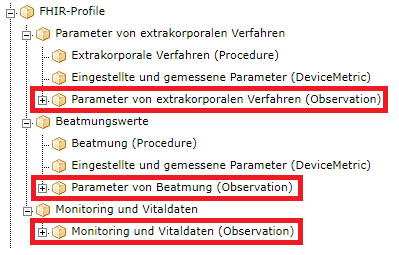
\includegraphics[height=8cm]{figures/icu_modul_tree_generics}
	\caption[Generische \glqq Observations\grqq{}]{Baumstruktur des Erweiterungsmoduls \glqq Intensivmedizin\grqq{}. Die generischen Profile der Kategorie \glqq Observations\grqq{} sind rot markiert.}
	\label{fig:icutreegenerics}
\end{figure}

Das Modul \glqq\ac{icu}\grqq{} mit 80 \ac{fhir}-Profilen ist das umfangreichste Modul der \ac{mii}. Von diesen Profilen könnte in diesem Projekt 39 einem Biosignalparameter zugeordnet werden (\ref{fig:profile}). Die Grunde dieses Ergebnisses sind nicht nur von dem Umfang des Modul abhängig, sondern von den Bioparameter im \ac{copra}-System (\ref{sec:configvarcopradiscu}).

\clearpage

\begin{figure}[ht]
	\centering
	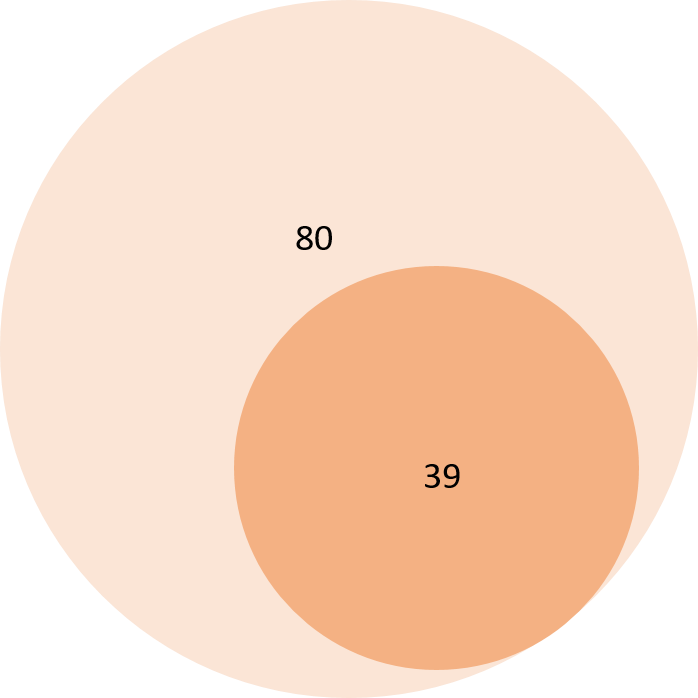
\includegraphics[height=7cm]{figures/profile}
	\caption[Diagramm der \acs{fhir}-Profile im Projekt]{Diagramm der \acs{fhir}-Profile im Projekt. Fast die Hälfte der \ac{fhir}-Profile konnten zugeordnet werden.}
	\label{fig:profile}
\end{figure}
